\documentclass[aspectratio=169]{beamer}
\usepackage[utf8]{inputenc}
\usepackage{xcolor}
\usepackage[ngerman]{babel}
\usepackage{siunitx}
\usepackage[european]{circuitikz}
\usepackage{pgfplots}
\usepackage{pdfpcnotes}

\usetheme{CambridgeUS}

\definecolor{toolboxOrange}{HTML}{f14531}

\setbeamercolor{section in toc}{fg=black,bg=white}
\setbeamercolor{alerted text}{fg=toolboxOrange}
\setbeamercolor*{palette primary}{fg=toolboxOrange,bg=gray!30!white}
\setbeamercolor*{palette secondary}{fg=toolboxOrange,bg=gray!15!white}
\setbeamercolor*{palette tertiary}{bg=toolboxOrange,fg=gray!10!white}
\setbeamercolor*{palette quaternary}{fg=toolboxOrange,bg=gray!5!white}
\setbeamercolor*{sidebar}{fg=toolboxOrange,bg=gray!15!white}
\setbeamercolor*{palette sidebar primary}{fg=toolboxOrange}
\setbeamercolor*{palette sidebar secondary}{fg=white}
\setbeamercolor*{palette sidebar tertiary}{fg=toolboxOrange}
\setbeamercolor*{palette sidebar quaternary}{fg=gray!10!white}
\setbeamercolor{titlelike}{parent=palette primary,fg=toolboxOrange}
\setbeamercolor{frametitle}{bg=gray!10!white}
\setbeamercolor{frametitle right}{bg=gray!60!white}

\pgfplotsset{ticks=none}

\pgfplotsset{every axis x label/.style={
  at={(0.5,0)},
  below,
  yshift=-5pt
  }
}

\pgfplotsset{every axis y label/.style={
  at={(0,0.5)},
  xshift=-15pt,
  rotate=90
  }
}

\pgfplotsset{compat=1.15}

\title{Praktischer Einstieg in die Elektronik}

\author{Paul Nykiel \and Jonas Otto}

\institute[Toolbox Bodensee]

\date{Toolbox Bodensee, \the\year}

\subject{Elektrotechnik}

\logo{
\includegraphics[height=0.13\textheight]{toolbox_logo_orange}}



\begin{document}

\begin{frame}
  \titlepage
\end{frame}

\section{Einführung} 
\begin{frame}{Wer sind wir?}
    \begin{columns}
        \begin{column}{0.5\textwidth}
            \begin{itemize}
                \item Teilnahme am RoboCup mit der Roboter-AG am Bildungszentrum
                \item Diverse elektronische Projekte in der Toolbox
                \item Studium der Informationssystemtechnik
                \item Aktuelles Projekt: Autonomes Modellflugzeug
            \end{itemize}
        \end{column}
        \begin{column}{0.5\textwidth}
            \begin{figure}
                \centering
                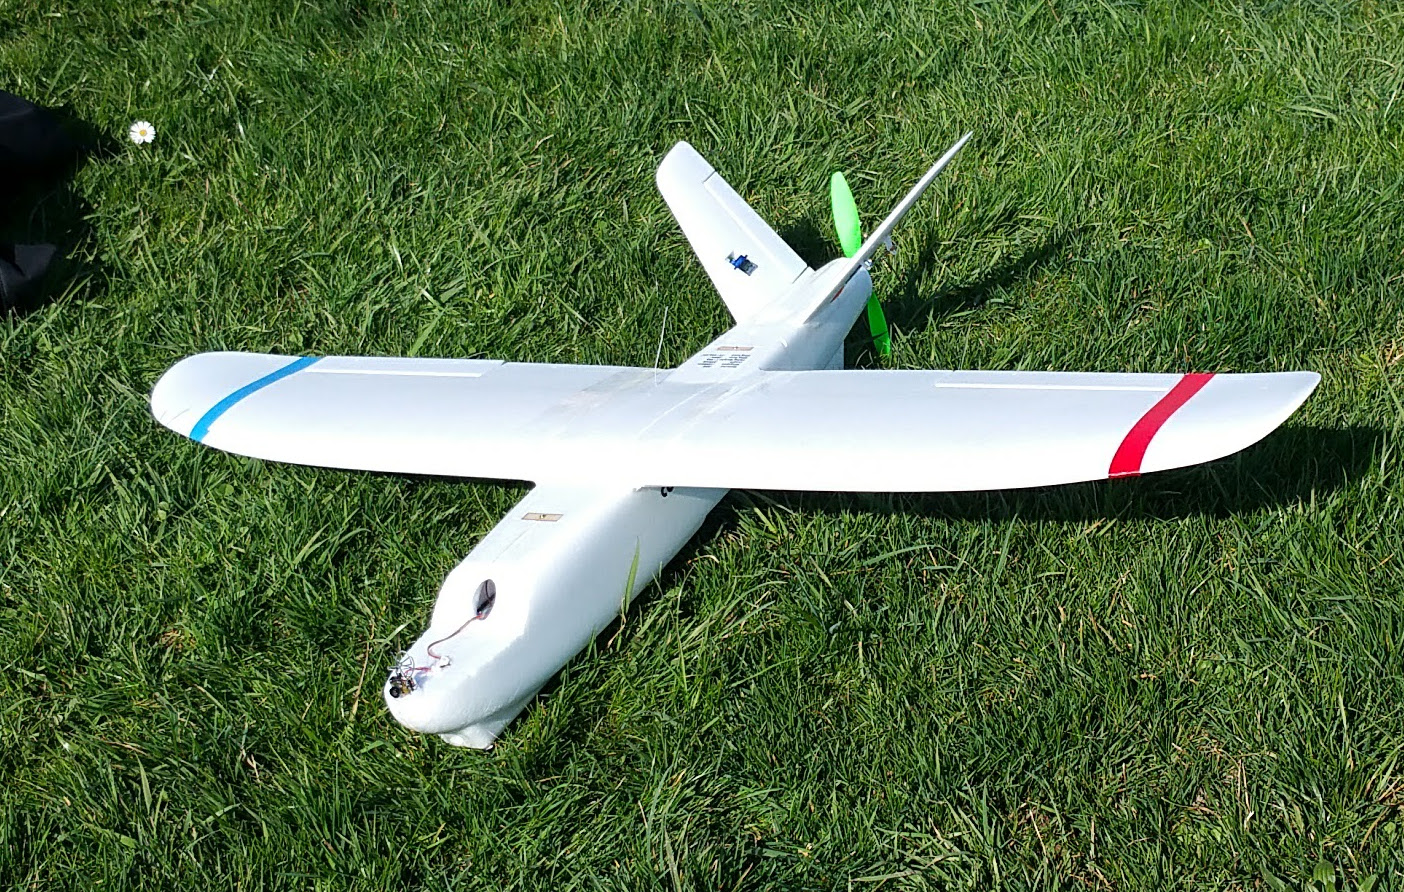
\includegraphics[width=0.8\textwidth]{20170329_155837.jpg}
                \caption{Autonomes Modellflugzeug}
            \end{figure} 
        \end{column}
    \end{columns}
\end{frame}

\section{Physik}

\begin{frame}{Strom}
    \begin{columns}
        \begin{column}{0.5\textwidth}
            Ladungsmenge, die in einer bestimmten Zeit durch einen Leiter \glqq{}fließt\grqq{} \\
            \pause
            $\Leftrightarrow$ Ladung pro Zeit
        \end{column}
        \pause
        \begin{column}{0.5\textwidth}
            \begin{block}{Strom}
                \begin{itemize}
                    \item Einheit: Ampere $[\si{A}]$
                    \item Formelzeichen: $I$
                    \item Typische Werte:
                        \begin{itemize}
                            \item Microcontroller: $<5 \si{mA}$
                            \item LED: $<30 \si{mA}$
                            \item Handyladegerät: $1-2\si{A}$
                            \item Quadrocoptermotor: $10-40 \si{A}$
                        \end{itemize}
                \end{itemize}
            \end{block}
        \end{column}
    \end{columns}
\end{frame}

\begin{frame}{Spannung} \begin{columns} 
\begin{column}{0.5\textwidth} 
Mit wieviel Druck werden die Ladungen durch den Leiter \glqq{}gedrückt\grqq{} \\ \pause $\Leftrightarrow$ \glqq{}Höhenunterschied\grqq{} zwischen zwei Punkten der Schaltung \\ \pause $\Leftrightarrow$
            Potentialdifferenz
        \end{column}
        \pause
        \begin{column}{0.5\textwidth}
            \begin{block}{Spannung}
                \begin{itemize}
                    \item Einheit: Volt $[\si{V}]$
                    \item Formelzeichen: $U$
                    \item Typische Werte: $3.3 \si{V}, 3.7 \si{V}, 5 \si{V}, 12 \si{V}$
                \end{itemize}
            \end{block}
        \end{column}
    \end{columns}
\end{frame}

\section{Bauelemente}

\subsection{Widerstand}
\begin{frame}{Widerstand}{Experiment}
    %\pnote{vlc --v4l2-width=1280 --v4l2-height=720 --v4l2-fps=30 --v4l2-chroma=mjpg -vv v4l2:///dev/video0}
    \pnote{Leistungswiderstand erwärmen, Kleinen THT Widerstand kaputtmachen}
    \begin{alertblock}{Vorsicht}
        Widerstände nur innerhalb der im Datenblatt angegeben Strom/Spannungsgrenzen betreiben!\\
        Die Leistung an Widerständen ist begrenzt (Typische Werte: $0.1\si{W} - 1\si{W}$)
    \end{alertblock}
\end{frame}

\begin{frame}{Widerstand}{Ohmsches Gesetz}
    \pnote{Wassermodell: Rohrdurchmesser, Selbst Kabel haben Widerstand}
    \begin{columns}
        \begin{column}{0.5\textwidth}
            \begin{itemize}
                \item Zusammenhang zwischen Strom und Spannung \pause 
                \item Widerstand ist feste Eigenschaft eines Leiters \pause
                \item Spannung Proportional zu Strom \pause 
            \end{itemize}
            \begin{equation*}
                U=R \cdot I
            \end{equation*}
            \pause
        \end{column}
        \begin{column}{0.5\textwidth}
            \begin{block}{Widerstand}
                \begin{itemize}
                    \item Einheit: Ohm $[\si{\ohm}]$
                    \item Formelzeichen: $R$
                    \item Schaltzeichen:
                        \begin{circuitikz}
                            \draw (0,0) to[R] (2,0);
                        \end{circuitikz}
                    \item Typische Werte: $1\si{k\ohm}$, $4.7\si{k\ohm}$, $10\si{k\ohm}$
                \end{itemize}
            \end{block}
        \end{column}
    \end{columns}
\end{frame}

\begin{frame}{Widerstand}{Experiment: Ohmsches Gesetz}
    \pnote{Verschiedene WIderstände an gleiche Spannung anschließen, Strom zeigen}
    \begin{center}
        {\huge Demonstration}
    \end{center}
\end{frame}

\begin{frame}{Widerstand}{Reihenschaltung}
    \begin{columns}
        \begin{column}{0.5\textwidth}
            \begin{figure}
                \centering
                 \resizebox{!}{0.3\textheight}{
                \begin{circuitikz}
                    \draw (0,2) to[R, l_=$R_1$] (0,4);
                    \draw (0,0) to[R, l_=$R_2$] (0,2);
                \end{circuitikz}}
                \caption{Reihenschaltung}
            \end{figure}
            \pause
            \begin{equation*}
                R_\text{Gesamt} = R_1 + R_2
            \end{equation*}
        \end{column}
        \pause
        \begin{column}{0.5\textwidth}
             \begin{figure}
                \centering
                 \resizebox{!}{0.3\textheight}{
                \begin{circuitikz}
                   \draw (0,1) to[R, l_=$R_1$] (0,3);
                   \draw (2,1) to[R, l_=$R_2$] (2,3);
                   \draw (0,1) -- (2,1);
                   \draw (1,1) -- (1,0);
                   \draw (0,3) -- (2,3);
                   \draw (1,3) -- (1,4);
                \end{circuitikz}}
                \caption{Parallelschaltung}
            \end{figure}
            %\pause
            %\begin{equation}
            %    \frac{1}{R_\text{Gesamt}} = \frac{1}{R_1} + \frac{1}{R_2}
            %\end{equation}
        \end{column}
    \end{columns}
\end{frame}

\begin{frame}{Widerstand}{Spannungsteiler}
    \pnote{Variabler Widerstand erklären, Nicht für Spannungswandlung!}
    \begin{columns}
        \begin{column}{0.5\textwidth}
        \begin{itemize}
            \item Die Spannungen an den Widerständen in einer Reihenschaltung sind Proportional zu den Widerständen \pause \\
            \item Nützlich für das Messen von Widerständen (z.B. Sensoren über die Spannung) \pause
        \end{itemize}
        \end{column}
        \begin{column}{0.5\textwidth}
            \begin{figure}[t]
                \centering
                \resizebox{!}{0.4\textheight}{
                \begin{circuitikz}
                    \draw (0,0) node[rground] {};
                    \draw (0,0) to[R] (0,2);
                    \draw (0,2) to[vR] (0,4);
                    \draw (0,4) node[vcc] {};
                    \draw (0,2) -- (1,2);
                \end{circuitikz}}
                \caption{Spannungsteiler}
            \end{figure}
        \end{column}
    \end{columns}
\end{frame}

\subsection{Verbraucher (Widerstand)}

\begin{frame}{Verbraucher (Widerstand)}
    Viele Verbraucher lassen sich als Widerstand modellieren:
    \begin{itemize}
        \item Glühlampe
        \item DC-Motor
    \end{itemize}
\end{frame}

\subsection{Kondensator}

\begin{frame}{Kondensator}{Experiment}
    \pnote{Elko verpolt an hohe Spannung}
    \begin{center}
        {\huge Demonstration}
    \end{center}
\end{frame}

\begin{frame}{Kondensator}
    \begin{columns}
        \begin{column}{0.5\textwidth}
        \begin{itemize}
            \item Ladungsspeicher \pause
            \item Braucht Zeit um ge-/entladen zu werden \pause
            \item Strom proportional zur Änderungsrate der Spannung \pause
        \end{itemize}
        $\Rightarrow$ Gedächtnissbehaftetes Bauteil \pause
        \end{column}
        \begin{column}{0.5\textwidth}
            \begin{block}{Kondensator}
                \begin{itemize}
                    \item Einheit: Farad $\si{F}$
                    \item Formelzeichen: $C$
                    \item Schaltzeichen:
                        \begin{circuitikz}
                            \draw (0,0) to[C] (2,0);
                        \end{circuitikz}
                    \item Typische Werte: $22 \si{pF}$, $100 \si{nF}$
                \end{itemize}
            \end{block}
        \end{column}
    \end{columns}
\end{frame}

\begin{frame}{Kondensator}{Experiment: Aufladen}
    \pnote{Kondensator durch Widerstand aufladen, zeigen dass Ladung erhalten bleibt}
    \begin{columns}
        \begin{column}{0.5\textwidth}
            \centering
            \begin{circuitikz}
                \draw (0,4) to[american voltage source] (0,0);
                \draw (0,4) to[switch] (3,4);
                \draw (3,4) to[R] (3,2);
                \draw (2,2) -- (4,2);
                \draw (0,0) -- (4,0);
                \draw (2,2) to[C] (2,0);
                \draw (4,2) to[lamp] (4,0);
            \end{circuitikz}
        \end{column}
        \pause
        \begin{column}{0.5\textwidth}
            \centering
            \begin{tikzpicture}
                \begin{axis}[ 
                    xlabel=$t$,
                    ylabel={$u(t)$},
                    xmin=0,
                    xmax=5,
                    ymin=0,
                    ymax=1,
                    width=\textwidth,
                    height=5cm,
                    thick,
                ] 
                \addplot [domain=0:5, color=toolboxOrange]{(1-e^(-x))}; 
                \end{axis}
            \end{tikzpicture}
        \end{column}
    \end{columns}
\end{frame}

\begin{frame}{Kondensator}{Experiment: Entladen}
    \pnote{Mit Glühlampe entladen}
    \begin{columns}
        \begin{column}{0.5\textwidth}
            \centering
            \begin{circuitikz}
                \draw (0,4) to[american voltage source] (0,0);
                \draw (0,4) to[opening switch] (3,4);
                \draw (3,4) to[R] (3,2);
                \draw (2,2) -- (4,2);
                \draw (0,0) -- (4,0);
                \draw (2,2) to[C] (2,0);
                \draw (4,2) to[lamp] (4,0);
            \end{circuitikz}
        \end{column}
        \pause
        \begin{column}{0.5\textwidth}
            \centering
            \begin{tikzpicture}
                \begin{axis}[ 
                    xlabel=$t$,
                    ylabel={$u(t)$},
                    xmin=0,
                    xmax=5,
                    ymin=0,
                    ymax=1,
                    width=\textwidth,
                    height=5cm,
                    thick,
                ] 
                \addplot [domain=0:5, color=toolboxOrange]{(e^(-x))}; 
                \end{axis}
            \end{tikzpicture}
        \end{column}
    \end{columns}
\end{frame}

\begin{frame}{Kapazitator}{Einsatz}
    Spannung am Kapazitator springt nicht \\ \pause
    $\Rightarrow$ Spannungspeaks und schnelle Spannungsänderungen werden vom Kapazitator geblockt
    \\ \pause
    $\Rightarrow$ Nur niedrige/tiefe Frequenzen werden vom Kapazitator durchgelassen
    \\ \pause
    $\Rightarrow$ Tiefpass \pause \\
    \centering
    \begin{tikzpicture}
        \begin{axis}[ 
            xlabel=$t$,
            ylabel={$u(t)$},
            xmin=0,
            xmax=5,
            ymin=-2,
            ymax=2,
            width=\textwidth,
            height=4cm,
            width=0.7\textwidth,
            thick,
        ] 
        \addplot [domain=0:5, color=toolboxOrange, samples=1000]{0.6*sin((x-0.5)*180)}; 
        \addplot [domain=0:5, color=toolboxOrange, dashed, samples=1000]{(-1)^floor(x)}; 
        \end{axis}
    \end{tikzpicture}
\end{frame}

\subsection{Spule}

\begin{frame}{Spule}
    \begin{columns}
        \begin{column}{0.5\textwidth}
            \begin{itemize}
                \item Ähnlich dem Kondensator \pause
                \item Spannung proportional zur Änderungsrate des Stroms \pause
                \item Hochpass \pause
            \end{itemize}
        \end{column}
        \begin{column}{0.5\textwidth}
            \begin{block}{Spule}
                \begin{itemize}
                    \item Einheit: Henry $[\si{H}]$
                    \item Formelzeichen: L
                    \item Schaltzeichen:
                        \begin{circuitikz}
                            \draw (0,0) to[L] (2,0);
                        \end{circuitikz}
                \end{itemize} 
            \end{block}
        \end{column}
    \end{columns}
\end{frame}

\section{Halbleiterbauelemente}

\subsection{Diode}

\begin{frame}{Diode}
    \begin{columns}
        \begin{column}{0.5\textwidth}
            Diode leitet nur in eine Richtung (Durchlassrichtung),\\
            in Sperrrichtung leitet die Diode nicht
        \end{column}
        \begin{column}{0.5\textwidth}
            \begin{block}{Diode}
                \begin{itemize}
                    \item Schaltzeichen:
                        \begin{circuitikz}
                            \draw (0,0) to[D] (2,0);
                        \end{circuitikz}
                \end{itemize} 
            \end{block}
        \end{column}
    \end{columns}
\end{frame}

\begin{frame}{Diode}{Experiment}
    \pnote{Kleine Diode in Glasgehäuse kaputtmachen}
    \begin{center}
        {\huge Demonstration}
    \end{center}
\end{frame}

\begin{frame}{Diode}{Brückengleichrichter}
    \begin{columns}
        \begin{column}{0.5\textwidth}
            Sperrwirkung kann zum \glqq{}Gleichrichten\grqq{} von Wechselspannung eingesetzt werden
        \end{column}
        \begin{column}{0.5\textwidth}
            \centering
            \begin{circuitikz}
                \draw (0,4) to[sinusoidal voltage source] (0,0);
                \draw (2,2) to[D] (3,1);
                \draw (3,3) to[D] (4,2);
                \draw (3,1) to[D] (4,2);
                \draw (2,2) to[D] (3,3);
                \draw (0,4) -- (3,4) -- (3,3);
                \draw (0,0) -- (3,0) -- (3,1);
                \draw (2,2) -- (1.5,2);
                \draw (1.5,2) node[anchor=east] {$-$};
                \draw (4,2) -- (4.5,2);
                \draw (4.5,2) node[anchor=west] {$+$};
            \end{circuitikz}
        \end{column}
    \end{columns}
\end{frame}

\subsection{LED}

\begin{frame}{LED}{Experiment: LED}
    \centering
    \begin{circuitikz}
        \draw (0,2) to[american voltage source] (0,0);
        \draw (0,2) to[R] (2,2);
        \draw (0,0) -- (2,0);
        \draw (2,2) to[empty led] (2,0);
    \end{circuitikz}
\end{frame}

\begin{frame}{LED}
    \begin{columns}
        \begin{column}{0.5\textwidth}
            \begin{itemize}
                \item Leitet in Durchlassrichtung $\Rightarrow$ Kurzschluss \pause
                \item Strom mit Widerstand begrenzen (Vorwiderstand) \pause
                \item Typischerweise maximal ca. $20\si{mA}$ \pause
            \end{itemize}
        \end{column}
        \begin{column}{0.5\textwidth}
            \begin{tikzpicture}
                \begin{axis}[ 
                    xlabel=$u$,
                    ylabel={$i(u)$},
                    xmin=0,
                    xmax=10,
                    ymin=0,
                    ymax=10,
                    width=\textwidth,
                    height=5cm,
                    thick,
                ]
                \addplot [domain=0:6, samples=500, color=toolboxOrange]{(exp(3*(x-4)))};
                \end{axis}
            \end{tikzpicture}
        \end{column}
    \end{columns}
\end{frame}

\subsection{Transistor}

\begin{frame}{Transistor}{Experiment}
\pnote{BC172 I_ce > 1A kaputtmachen}
    \begin{center}
        {\huge Demonstration}
    \end{center}
\end{frame}

\begin{frame}{Transistor}
    \begin{columns}
        \begin{column}{0.5\textwidth}
            \begin{itemize}
                \item Elektrisch steuerbarer Schalter
                \item Zentraler Bauteil von Computern
                \item Verschieden Typen: PNP, NPN, FET
            \end{itemize}
        \end{column}
        \begin{column}{0.5\textwidth}
            \begin{block}{Transistor}
                \begin{itemize}
                    \item Schaltbild:
                        \begin{circuitikz}
                            \draw (0,0) node[npn] at (0,0) {};
                        \end{circuitikz}
                \end{itemize}
            \end{block}
        \end{column}
    \end{columns}
\end{frame}

\begin{frame}{Transistor}{Experiment: Anwendung}
    \pnote{Motor Schalten mit Transistor} 
    \begin{columns}
        \begin{column}{0.5\textwidth}
            Mit wenig Strom/Spannung viel Strom/Spannung schalten
        \end{column}
        \begin{column}{0.5\textwidth}
            \centering
            \begin{circuitikz}
                \draw (0,0) node[npn](npn) at (0,0) {};
                \draw (npn.C) node[vcc]{};
                \draw (npn.E) --++(0,-0.5) node[elmech]{M} --++(0,-0.5) node[ground]{};
                \draw (npn.B) to[short, -o] ++(-1,0);
            \end{circuitikz}
        \end{column}
    \end{columns}
\end{frame}

\section{}
\subsection{}
\begin{frame}{}
    \begin{center}
        {\Huge Vielen Dank für eure Aufmerksamkeit!}
        
        \vspace{0.8cm}
        
        {\huge Gibt es noch Fragen?}
    \end{center}
\end{frame}

\end{document}